\documentclass{standalone}
\usepackage{tikz}
\usetikzlibrary{patterns, positioning}
\usepackage[sfdefault]{ClearSans} %% option 'sfdefault' activates Clear Sans as the default text font
\usepackage[T1]{fontenc}

\begin{document}
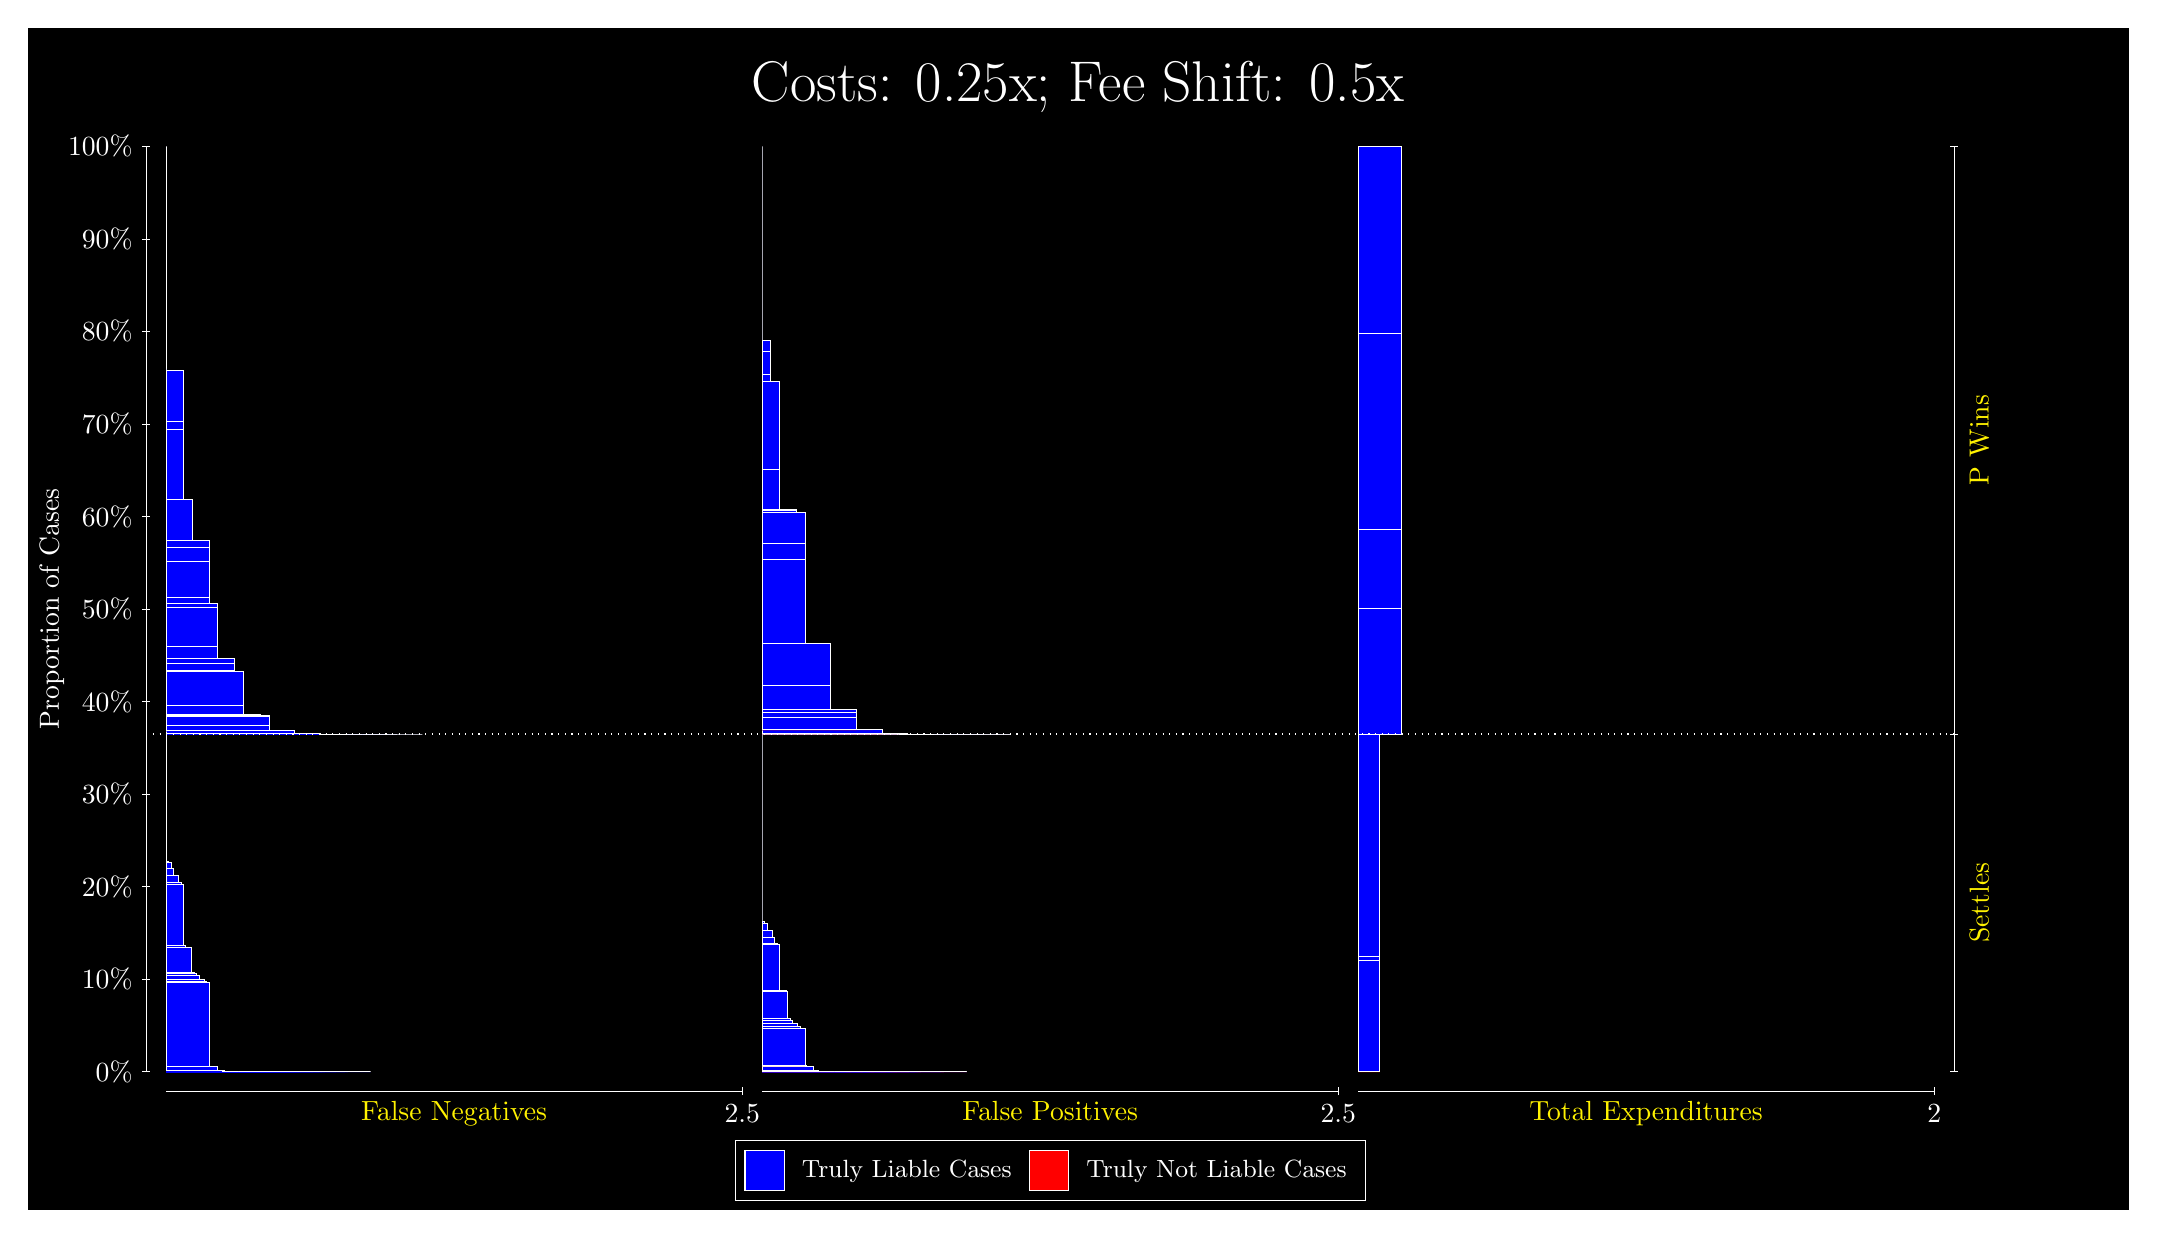
\begin{tikzpicture}
\draw[fill=black] (0,0) rectangle (26.667,15);
\draw[text=white] (0,13.5) rectangle (26.667,15) node[midway] {\huge Costs: 0.25x; Fee Shift: 0.5x};
\draw[white, very thin] (1.5,1.75) -- (1.5,13.5);
\node[rotate=90, text=white, anchor=center] at (0.3, 7.625) {Proportion of Cases};
\draw[white, very thin] (1.45,1.75) -- (1.55,1.75);
\node[text=white, anchor=east] at (1.45, 1.75) {0\%};
\draw[white, very thin] (1.45,2.925) -- (1.55,2.925);
\node[text=white, anchor=east] at (1.45, 2.925) {10\%};
\draw[white, very thin] (1.45,4.1) -- (1.55,4.1);
\node[text=white, anchor=east] at (1.45, 4.1) {20\%};
\draw[white, very thin] (1.45,5.275) -- (1.55,5.275);
\node[text=white, anchor=east] at (1.45, 5.275) {30\%};
\draw[white, very thin] (1.45,6.45) -- (1.55,6.45);
\node[text=white, anchor=east] at (1.45, 6.45) {40\%};
\draw[white, very thin] (1.45,7.625) -- (1.55,7.625);
\node[text=white, anchor=east] at (1.45, 7.625) {50\%};
\draw[white, very thin] (1.45,8.8) -- (1.55,8.8);
\node[text=white, anchor=east] at (1.45, 8.8) {60\%};
\draw[white, very thin] (1.45,9.975) -- (1.55,9.975);
\node[text=white, anchor=east] at (1.45, 9.975) {70\%};
\draw[white, very thin] (1.45,11.15) -- (1.55,11.15);
\node[text=white, anchor=east] at (1.45, 11.15) {80\%};
\draw[white, very thin] (1.45,12.325) -- (1.55,12.325);
\node[text=white, anchor=east] at (1.45, 12.325) {90\%};
\draw[white, very thin] (1.45,13.5) -- (1.55,13.5);
\node[text=white, anchor=east] at (1.45, 13.5) {100\%};

\draw[white, very thin] (24.457,1.75) -- (24.457,13.5);
\draw[white, very thin] (24.407,1.75) -- (24.507,1.75);
\node[anchor=west] at (24.407, 1.75) {};
\draw[white, very thin] (24.407,6.0366) -- (24.507,6.0366);
\node[anchor=west] at (24.407, 6.0366) {};
\draw[white, very thin] (24.407,13.5) -- (24.507,13.5);
\node[anchor=west] at (24.407, 13.5) {};

\draw[white, very thin, fill=blue] (1.75,1.75) rectangle (4.3482,1.75);
\draw[white, very thin, fill=blue] (1.75,1.75) rectangle (4.0554,1.75);
\draw[white, very thin, fill=blue] (1.75,1.75) rectangle (4.0229,1.75);
\draw[white, very thin, fill=blue] (1.75,1.75) rectangle (3.9091,1.75);
\draw[white, very thin, fill=blue] (1.75,1.75) rectangle (3.7627,1.75);
\draw[white, very thin, fill=blue] (1.75,1.75) rectangle (3.7302,1.75);
\draw[white, very thin, fill=blue] (1.75,1.75) rectangle (3.6976,1.75);
\draw[white, very thin, fill=blue] (1.75,1.75) rectangle (3.6163,1.75);
\draw[white, very thin, fill=blue] (1.75,1.75) rectangle (3.5838,1.75);
\draw[white, very thin, fill=blue] (1.75,1.75) rectangle (3.4699,1.75);
\draw[white, very thin, fill=blue] (1.75,1.75) rectangle (3.4374,1.75);
\draw[white, very thin, fill=blue] (1.75,1.75) rectangle (3.4049,1.75);
\draw[white, very thin, fill=blue] (1.75,1.75) rectangle (3.3723,1.75);
\draw[white, very thin, fill=blue] (1.75,1.75) rectangle (3.3236,1.75);
\draw[white, very thin, fill=blue] (1.75,1.75) rectangle (3.291,1.75);
\draw[white, very thin, fill=blue] (1.75,1.75) rectangle (3.2585,1.75);
\draw[white, very thin, fill=blue] (1.75,1.75) rectangle (3.1772,1.75);
\draw[white, very thin, fill=blue] (1.75,1.75) rectangle (3.1447,1.75);
\draw[white, very thin, fill=blue] (1.75,1.75) rectangle (3.1121,1.75);
\draw[white, very thin, fill=blue] (1.75,1.75) rectangle (3.0796,1.75);
\draw[white, very thin, fill=blue] (1.75,1.75) rectangle (3.0471,1.75);
\draw[white, very thin, fill=blue] (1.75,1.75) rectangle (3.0308,1.75);
\draw[white, very thin, fill=blue] (1.75,1.75) rectangle (2.9983,1.75);
\draw[white, very thin, fill=blue] (1.75,1.75) rectangle (2.9657,1.75);
\draw[white, very thin, fill=blue] (1.75,1.75) rectangle (2.9332,1.75);
\draw[white, very thin, fill=blue] (1.75,1.75) rectangle (2.8844,1.7501);
\draw[white, very thin, fill=blue] (1.75,1.7501) rectangle (2.8519,1.7501);
\draw[white, very thin, fill=blue] (1.75,1.7501) rectangle (2.8194,1.7501);
\draw[white, very thin, fill=blue] (1.75,1.7501) rectangle (2.7868,1.7502);
\draw[white, very thin, fill=blue] (1.75,1.7502) rectangle (2.7543,1.7502);
\draw[white, very thin, fill=blue] (1.75,1.7502) rectangle (2.7218,1.7525);
\draw[white, very thin, fill=blue] (1.75,1.7525) rectangle (2.7055,1.7525);
\draw[white, very thin, fill=blue] (1.75,1.7525) rectangle (2.673,1.7525);
\draw[white, very thin, fill=blue] (1.75,1.7525) rectangle (2.6405,1.7526);
\draw[white, very thin, fill=blue] (1.75,1.7526) rectangle (2.6079,1.7528);
\draw[white, very thin, fill=blue] (1.75,1.7528) rectangle (2.5917,1.7532);
\draw[white, very thin, fill=blue] (1.75,1.7532) rectangle (2.5591,1.7552);
\draw[white, very thin, fill=blue] (1.75,1.7552) rectangle (2.5266,1.7553);
\draw[white, very thin, fill=blue] (1.75,1.7553) rectangle (2.4941,1.7597);
\draw[white, very thin, fill=blue] (1.75,1.7597) rectangle (2.4616,1.7614);
\draw[white, very thin, fill=blue] (1.75,1.7614) rectangle (2.429,1.7642);
\draw[white, very thin, fill=blue] (1.75,1.7642) rectangle (2.3965,1.8178);
\draw[white, very thin, fill=blue] (1.75,1.8178) rectangle (2.3802,1.8178);
\draw[white, very thin, fill=blue] (1.75,1.8178) rectangle (2.3477,1.8179);
\draw[white, very thin, fill=blue] (1.75,1.8179) rectangle (2.3152,1.8223);
\draw[white, very thin, fill=blue] (1.75,1.8223) rectangle (2.2989,2.8834);
\draw[white, very thin, fill=blue] (1.75,2.8834) rectangle (2.2827,2.8856);
\draw[white, very thin, fill=blue] (1.75,2.8856) rectangle (2.2664,2.8908);
\draw[white, very thin, fill=blue] (1.75,2.8908) rectangle (2.2339,2.9213);
\draw[white, very thin, fill=blue] (1.75,2.9213) rectangle (2.2013,2.923);
\draw[white, very thin, fill=blue] (1.75,2.923) rectangle (2.1688,2.9674);
\draw[white, very thin, fill=blue] (1.75,2.9674) rectangle (2.1363,2.9947);
\draw[white, very thin, fill=blue] (1.75,2.9947) rectangle (2.1037,3.0136);
\draw[white, very thin, fill=blue] (1.75,3.0136) rectangle (2.0712,3.3252);
\draw[white, very thin, fill=blue] (1.75,3.3252) rectangle (2.055,3.3253);
\draw[white, very thin, fill=blue] (1.75,3.3253) rectangle (2.0224,3.3257);
\draw[white, very thin, fill=blue] (1.75,3.3257) rectangle (1.9899,3.3473);
\draw[white, very thin, fill=blue] (1.75,3.3473) rectangle (1.9736,4.1286);
\draw[white, very thin, fill=blue] (1.75,4.1286) rectangle (1.9574,4.1338);
\draw[white, very thin, fill=blue] (1.75,4.1338) rectangle (1.9411,4.1577);
\draw[white, very thin, fill=blue] (1.75,4.1577) rectangle (1.9086,4.2441);
\draw[white, very thin, fill=blue] (1.75,4.2441) rectangle (1.876,4.2484);
\draw[white, very thin, fill=blue] (1.75,4.2484) rectangle (1.8435,4.3343);
\draw[white, very thin, fill=blue] (1.75,4.3343) rectangle (1.811,4.403);
\draw[white, very thin, fill=blue] (1.75,4.403) rectangle (1.7785,4.4248);
\draw[white, very thin, fill=red] (1.75,4.4248) rectangle (1.75,4.4248);
\draw[white, very thin, fill=blue] (1.75,4.4248) rectangle (1.75,6.0366);
\draw[white, very thin, fill=blue] (1.75,6.0366) rectangle (5.0069,6.0366);
\draw[white, very thin, fill=blue] (1.75,6.0366) rectangle (4.6816,6.0366);
\draw[white, very thin, fill=blue] (1.75,6.0366) rectangle (4.5718,6.0366);
\draw[white, very thin, fill=blue] (1.75,6.0366) rectangle (4.3563,6.0366);
\draw[white, very thin, fill=blue] (1.75,6.0366) rectangle (4.2465,6.0366);
\draw[white, very thin, fill=blue] (1.75,6.0366) rectangle (4.2465,6.0366);
\draw[white, very thin, fill=blue] (1.75,6.0366) rectangle (4.031,6.0367);
\draw[white, very thin, fill=blue] (1.75,6.0367) rectangle (4.031,6.0369);
\draw[white, very thin, fill=blue] (1.75,6.0369) rectangle (3.9213,6.0369);
\draw[white, very thin, fill=blue] (1.75,6.0369) rectangle (3.7058,6.0395);
\draw[white, very thin, fill=blue] (1.75,6.0395) rectangle (3.7058,6.0413);
\draw[white, very thin, fill=blue] (1.75,6.0413) rectangle (3.596,6.0413);
\draw[white, very thin, fill=blue] (1.75,6.0413) rectangle (3.3805,6.0798);
\draw[white, very thin, fill=blue] (1.75,6.0798) rectangle (3.2707,6.0798);
\draw[white, very thin, fill=blue] (1.75,6.0798) rectangle (3.2707,6.08);
\draw[white, very thin, fill=blue] (1.75,6.08) rectangle (3.0552,6.1487);
\draw[white, very thin, fill=blue] (1.75,6.1487) rectangle (3.0552,6.2636);
\draw[white, very thin, fill=blue] (1.75,6.2636) rectangle (3.0552,6.2772);
\draw[white, very thin, fill=blue] (1.75,6.2772) rectangle (2.9454,6.2805);
\draw[white, very thin, fill=blue] (1.75,6.2805) rectangle (2.9454,6.2876);
\draw[white, very thin, fill=blue] (1.75,6.2876) rectangle (2.9454,6.2914);
\draw[white, very thin, fill=blue] (1.75,6.2914) rectangle (2.7299,6.4012);
\draw[white, very thin, fill=blue] (1.75,6.4012) rectangle (2.7299,6.8309);
\draw[white, very thin, fill=blue] (1.75,6.8309) rectangle (2.6201,6.8396);
\draw[white, very thin, fill=blue] (1.75,6.8396) rectangle (2.6201,6.9316);
\draw[white, very thin, fill=blue] (1.75,6.9316) rectangle (2.6201,7.0025);
\draw[white, very thin, fill=blue] (1.75,7.0025) rectangle (2.4046,7.1517);
\draw[white, very thin, fill=blue] (1.75,7.1517) rectangle (2.4046,7.6499);
\draw[white, very thin, fill=blue] (1.75,7.6499) rectangle (2.4046,7.6918);
\draw[white, very thin, fill=blue] (1.75,7.6918) rectangle (2.2948,7.7679);
\draw[white, very thin, fill=blue] (1.75,7.7679) rectangle (2.2948,8.2335);
\draw[white, very thin, fill=blue] (1.75,8.2335) rectangle (2.2948,8.4055);
\draw[white, very thin, fill=blue] (1.75,8.4055) rectangle (2.2948,8.5023);
\draw[white, very thin, fill=blue] (1.75,8.5023) rectangle (2.0793,9.016);
\draw[white, very thin, fill=blue] (1.75,9.016) rectangle (1.9696,9.9086);
\draw[white, very thin, fill=blue] (1.75,9.9086) rectangle (1.9696,10.003);
\draw[white, very thin, fill=blue] (1.75,10.003) rectangle (1.9696,10.651);
\draw[white, very thin, fill=blue] (1.75,10.651) rectangle (1.7541,10.678);
\draw[white, very thin, fill=blue] (1.75,10.678) rectangle (1.7541,10.678);
\draw[white, very thin, fill=red] (1.75,10.678) rectangle (1.75,10.678);
\draw[white, very thin, fill=blue] (1.75,10.678) rectangle (1.75,13.5);
\draw[white, very thin, fill=red] (9.3189,1.75) rectangle (11.917,1.75);
\draw[white, very thin, fill=blue] (9.3189,1.75) rectangle (11.917,1.75);
\draw[white, very thin, fill=red] (9.3189,1.75) rectangle (11.624,1.75);
\draw[white, very thin, fill=blue] (9.3189,1.75) rectangle (11.624,1.75);
\draw[white, very thin, fill=blue] (9.3189,1.75) rectangle (11.592,1.75);
\draw[white, very thin, fill=red] (9.3189,1.75) rectangle (11.332,1.75);
\draw[white, very thin, fill=blue] (9.3189,1.75) rectangle (11.332,1.75);
\draw[white, very thin, fill=blue] (9.3189,1.75) rectangle (11.299,1.75);
\draw[white, very thin, fill=blue] (9.3189,1.75) rectangle (11.266,1.75);
\draw[white, very thin, fill=red] (9.3189,1.75) rectangle (11.185,1.75);
\draw[white, very thin, fill=blue] (9.3189,1.75) rectangle (11.185,1.75);
\draw[white, very thin, fill=red] (9.3189,1.75) rectangle (11.039,1.75);
\draw[white, very thin, fill=blue] (9.3189,1.75) rectangle (11.039,1.75);
\draw[white, very thin, fill=blue] (9.3189,1.75) rectangle (11.006,1.75);
\draw[white, very thin, fill=blue] (9.3189,1.75) rectangle (10.974,1.75);
\draw[white, very thin, fill=blue] (9.3189,1.75) rectangle (10.941,1.75);
\draw[white, very thin, fill=red] (9.3189,1.75) rectangle (10.892,1.75);
\draw[white, very thin, fill=blue] (9.3189,1.75) rectangle (10.892,1.75);
\draw[white, very thin, fill=blue] (9.3189,1.75) rectangle (10.86,1.75);
\draw[white, very thin, fill=red] (9.3189,1.75) rectangle (10.746,1.75);
\draw[white, very thin, fill=blue] (9.3189,1.75) rectangle (10.746,1.75);
\draw[white, very thin, fill=blue] (9.3189,1.75) rectangle (10.714,1.75);
\draw[white, very thin, fill=blue] (9.3189,1.75) rectangle (10.681,1.75);
\draw[white, very thin, fill=blue] (9.3189,1.75) rectangle (10.648,1.75);
\draw[white, very thin, fill=blue] (9.3189,1.75) rectangle (10.616,1.75);
\draw[white, very thin, fill=red] (9.3189,1.75) rectangle (10.6,1.75);
\draw[white, very thin, fill=blue] (9.3189,1.75) rectangle (10.6,1.75);
\draw[white, very thin, fill=blue] (9.3189,1.75) rectangle (10.567,1.75);
\draw[white, very thin, fill=blue] (9.3189,1.75) rectangle (10.535,1.75);
\draw[white, very thin, fill=red] (9.3189,1.75) rectangle (10.453,1.75);
\draw[white, very thin, fill=blue] (9.3189,1.75) rectangle (10.453,1.7501);
\draw[white, very thin, fill=blue] (9.3189,1.7501) rectangle (10.421,1.7501);
\draw[white, very thin, fill=blue] (9.3189,1.7501) rectangle (10.388,1.7501);
\draw[white, very thin, fill=blue] (9.3189,1.7501) rectangle (10.356,1.7502);
\draw[white, very thin, fill=blue] (9.3189,1.7502) rectangle (10.323,1.7503);
\draw[white, very thin, fill=red] (9.3189,1.7503) rectangle (10.307,1.7503);
\draw[white, very thin, fill=blue] (9.3189,1.7503) rectangle (10.307,1.7503);
\draw[white, very thin, fill=blue] (9.3189,1.7503) rectangle (10.291,1.7526);
\draw[white, very thin, fill=blue] (9.3189,1.7526) rectangle (10.274,1.7527);
\draw[white, very thin, fill=blue] (9.3189,1.7527) rectangle (10.242,1.7527);
\draw[white, very thin, fill=blue] (9.3189,1.7527) rectangle (10.209,1.7527);
\draw[white, very thin, fill=red] (9.3189,1.7527) rectangle (10.161,1.7527);
\draw[white, very thin, fill=blue] (9.3189,1.7527) rectangle (10.161,1.753);
\draw[white, very thin, fill=blue] (9.3189,1.753) rectangle (10.128,1.755);
\draw[white, very thin, fill=blue] (9.3189,1.755) rectangle (10.095,1.7567);
\draw[white, very thin, fill=blue] (9.3189,1.7567) rectangle (10.063,1.7569);
\draw[white, very thin, fill=blue] (9.3189,1.7569) rectangle (10.03,1.7613);
\draw[white, very thin, fill=blue] (9.3189,1.7613) rectangle (9.9979,1.7659);
\draw[white, very thin, fill=blue] (9.3189,1.7659) rectangle (9.9816,1.7661);
\draw[white, very thin, fill=blue] (9.3189,1.7661) rectangle (9.9654,1.8202);
\draw[white, very thin, fill=blue] (9.3189,1.8202) rectangle (9.9491,1.823);
\draw[white, very thin, fill=blue] (9.3189,1.823) rectangle (9.9166,1.823);
\draw[white, very thin, fill=blue] (9.3189,1.823) rectangle (9.884,1.8231);
\draw[white, very thin, fill=red] (9.3189,1.8231) rectangle (9.8678,1.8231);
\draw[white, very thin, fill=blue] (9.3189,1.8231) rectangle (9.8678,2.2963);
\draw[white, very thin, fill=blue] (9.3189,2.2963) rectangle (9.8353,2.3014);
\draw[white, very thin, fill=blue] (9.3189,2.3014) rectangle (9.8027,2.329);
\draw[white, very thin, fill=blue] (9.3189,2.329) rectangle (9.7702,2.359);
\draw[white, very thin, fill=blue] (9.3189,2.359) rectangle (9.7377,2.3607);
\draw[white, very thin, fill=blue] (9.3189,2.3607) rectangle (9.7051,2.4056);
\draw[white, very thin, fill=blue] (9.3189,2.4056) rectangle (9.6726,2.4292);
\draw[white, very thin, fill=blue] (9.3189,2.4292) rectangle (9.6563,2.4315);
\draw[white, very thin, fill=blue] (9.3189,2.4315) rectangle (9.6401,2.7649);
\draw[white, very thin, fill=blue] (9.3189,2.7649) rectangle (9.6238,2.7838);
\draw[white, very thin, fill=blue] (9.3189,2.7838) rectangle (9.5913,2.7843);
\draw[white, very thin, fill=blue] (9.3189,2.7843) rectangle (9.5588,2.7843);
\draw[white, very thin, fill=blue] (9.3189,2.7843) rectangle (9.5425,3.3619);
\draw[white, very thin, fill=blue] (9.3189,3.3619) rectangle (9.51,3.3836);
\draw[white, very thin, fill=blue] (9.3189,3.3836) rectangle (9.4774,3.4523);
\draw[white, very thin, fill=blue] (9.3189,3.4523) rectangle (9.4449,3.5382);
\draw[white, very thin, fill=blue] (9.3189,3.5382) rectangle (9.4124,3.5425);
\draw[white, very thin, fill=blue] (9.3189,3.5425) rectangle (9.3799,3.6289);
\draw[white, very thin, fill=blue] (9.3189,3.6289) rectangle (9.3473,3.6528);
\draw[white, very thin, fill=blue] (9.3189,3.6528) rectangle (9.3311,3.658);
\draw[white, very thin, fill=blue] (9.3189,3.658) rectangle (9.3189,6.0366);
\draw[white, very thin, fill=red] (9.3189,6.0366) rectangle (12.466,6.0366);
\draw[white, very thin, fill=blue] (9.3189,6.0366) rectangle (12.466,6.0366);
\draw[white, very thin, fill=red] (9.3189,6.0366) rectangle (12.141,6.0366);
\draw[white, very thin, fill=blue] (9.3189,6.0366) rectangle (12.141,6.0366);
\draw[white, very thin, fill=red] (9.3189,6.0366) rectangle (11.815,6.0366);
\draw[white, very thin, fill=blue] (9.3189,6.0366) rectangle (11.815,6.0366);
\draw[white, very thin, fill=blue] (9.3189,6.0366) rectangle (11.815,6.0366);
\draw[white, very thin, fill=blue] (9.3189,6.0366) rectangle (11.49,6.0368);
\draw[white, very thin, fill=red] (9.3189,6.0368) rectangle (11.49,6.0368);
\draw[white, very thin, fill=blue] (9.3189,6.0368) rectangle (11.49,6.0371);
\draw[white, very thin, fill=red] (9.3189,6.0371) rectangle (11.165,6.0371);
\draw[white, very thin, fill=blue] (9.3189,6.0371) rectangle (11.165,6.0428);
\draw[white, very thin, fill=red] (9.3189,6.0428) rectangle (11.055,6.0428);
\draw[white, very thin, fill=blue] (9.3189,6.0428) rectangle (11.055,6.0428);
\draw[white, very thin, fill=red] (9.3189,6.0428) rectangle (10.84,6.0428);
\draw[white, very thin, fill=blue] (9.3189,6.0428) rectangle (10.84,6.0915);
\draw[white, very thin, fill=blue] (9.3189,6.0915) rectangle (10.73,6.0915);
\draw[white, very thin, fill=red] (9.3189,6.0915) rectangle (10.73,6.0915);
\draw[white, very thin, fill=blue] (9.3189,6.0915) rectangle (10.73,6.0915);
\draw[white, very thin, fill=red] (9.3189,6.0915) rectangle (10.514,6.0915);
\draw[white, very thin, fill=blue] (9.3189,6.0915) rectangle (10.514,6.2434);
\draw[white, very thin, fill=blue] (9.3189,6.2434) rectangle (10.514,6.3076);
\draw[white, very thin, fill=blue] (9.3189,6.3076) rectangle (10.514,6.3482);
\draw[white, very thin, fill=blue] (9.3189,6.3482) rectangle (10.404,6.3482);
\draw[white, very thin, fill=red] (9.3189,6.3482) rectangle (10.404,6.3482);
\draw[white, very thin, fill=blue] (9.3189,6.3482) rectangle (10.404,6.3482);
\draw[white, very thin, fill=red] (9.3189,6.3482) rectangle (10.189,6.3482);
\draw[white, very thin, fill=blue] (9.3189,6.3482) rectangle (10.189,6.6589);
\draw[white, very thin, fill=blue] (9.3189,6.6589) rectangle (10.189,7.1894);
\draw[white, very thin, fill=blue] (9.3189,7.1894) rectangle (10.079,7.1894);
\draw[white, very thin, fill=red] (9.3189,7.1894) rectangle (10.079,7.1894);
\draw[white, very thin, fill=blue] (9.3189,7.1894) rectangle (10.079,7.1895);
\draw[white, very thin, fill=red] (9.3189,7.1895) rectangle (9.8637,7.1895);
\draw[white, very thin, fill=blue] (9.3189,7.1895) rectangle (9.8637,8.2556);
\draw[white, very thin, fill=blue] (9.3189,8.2556) rectangle (9.8637,8.4589);
\draw[white, very thin, fill=blue] (9.3189,8.4589) rectangle (9.8637,8.8585);
\draw[white, very thin, fill=blue] (9.3189,8.8585) rectangle (9.7539,8.8586);
\draw[white, very thin, fill=red] (9.3189,8.8586) rectangle (9.7539,8.8586);
\draw[white, very thin, fill=blue] (9.3189,8.8586) rectangle (9.7539,8.8756);
\draw[white, very thin, fill=blue] (9.3189,8.8756) rectangle (9.7539,8.8859);
\draw[white, very thin, fill=blue] (9.3189,8.8859) rectangle (9.5384,9.3955);
\draw[white, very thin, fill=blue] (9.3189,9.3955) rectangle (9.5384,10.521);
\draw[white, very thin, fill=blue] (9.3189,10.521) rectangle (9.4287,10.609);
\draw[white, very thin, fill=red] (9.3189,10.609) rectangle (9.4287,10.609);
\draw[white, very thin, fill=blue] (9.3189,10.609) rectangle (9.4287,10.9);
\draw[white, very thin, fill=blue] (9.3189,10.9) rectangle (9.4287,11.034);
\draw[white, very thin, fill=blue] (9.3189,11.034) rectangle (9.3189,13.5);
\draw[white, very thin, fill=red] (16.888,1.75) rectangle (17.162,1.75);
\draw[white, very thin, fill=blue] (16.888,1.75) rectangle (17.162,3.1684);
\draw[white, very thin, fill=red] (16.888,3.1684) rectangle (17.162,3.1684);
\draw[white, very thin, fill=blue] (16.888,3.1684) rectangle (17.162,3.2173);
\draw[white, very thin, fill=red] (16.888,3.2173) rectangle (17.162,3.2173);
\draw[white, very thin, fill=blue] (16.888,3.2173) rectangle (17.162,6.0366);
\draw[white, very thin, fill=red] (16.888,6.0366) rectangle (17.437,6.0366);
\draw[white, very thin, fill=blue] (16.888,6.0366) rectangle (17.437,7.6347);
\draw[white, very thin, fill=red] (16.888,7.6347) rectangle (17.437,7.6347);
\draw[white, very thin, fill=blue] (16.888,7.6347) rectangle (17.437,8.6413);
\draw[white, very thin, fill=red] (16.888,8.6413) rectangle (17.437,8.6413);
\draw[white, very thin, fill=blue] (16.888,8.6413) rectangle (17.437,11.125);
\draw[white, very thin, fill=red] (16.888,11.125) rectangle (17.437,11.125);
\draw[white, very thin, fill=blue] (16.888,11.125) rectangle (17.437,13.5);
\draw[white, dotted] (1.5,6.0366) -- (24.457,6.0366);
\draw[white, very thin] (1.75,1.5) -- (9.0689,1.5);
\node[text=yellow, anchor=north] at (5.4094, 1.5) {False Negatives};
\draw[white, very thin] (9.0689,1.45) -- (9.0689,1.55);
\node[text=white, anchor=north] at (9.0689, 1.45) {2.5};

\draw[white, very thin] (9.3189,1.5) -- (16.638,1.5);
\node[text=yellow, anchor=north] at (12.978, 1.5) {False Positives};
\draw[white, very thin] (16.638,1.45) -- (16.638,1.55);
\node[text=white, anchor=north] at (16.638, 1.45) {2.5};

\draw[white, very thin] (16.888,1.5) -- (24.207,1.5);
\node[text=yellow, anchor=north] at (20.547, 1.5) {Total Expenditures};
\draw[white, very thin] (24.207,1.45) -- (24.207,1.55);
\node[text=white, anchor=north] at (24.207, 1.45) {2};

\node[text=yellow, centered, rotate=90] at (24.777, 3.8933) {Settles};
\node[text=yellow, centered, rotate=90] at (24.777, 9.7683) {P Wins};

\draw (12.978300999999998,1.5) node[draw=none] (baseCoordinate) {};
\begin{scope}[align=center]
        \matrix[scale=0.5, draw=white, below=0.5cm of baseCoordinate, nodes={draw}, column sep=0.1cm]{
            \node[rectangle, draw, minimum width=0.5cm, minimum height=0.5cm, fill=blue] {}; &
            \node[draw=none, font=\small, text=white] (B) {Truly Liable Cases}; &
            \node[rectangle, draw, minimum width=0.5cm, minimum height=0.5cm, fill=red] {}; &
            \node[draw=none, font=\small, text=white] (B) {Truly Not Liable Cases}; \\
            };
\end{scope}

\end{tikzpicture}
\end{document}